\documentclass[10pt, letterpaper] {article}
%\documentclass{article}
%\usepackage{biblatex}
%\usepackage{apacite}
\usepackage{natbib}
\usepackage{amsmath, amsthm, amssymb, mathrsfs,array}
\usepackage{graphicx,float,wrapfig,subfigure,color,pdfpages,fixltx2e,url}
\pagestyle{plain}
\setlength{\parskip} {11pt}
\setlength{\parindent} {2em}
\setlength{\textwidth}{6.5in}
\setlength{\oddsidemargin} {0in}
\setlength{\textheight} {8.5in}
\setlength{\topmargin} {-0.5in}
\parskip 7.2pt

\newcommand{\nnub}{\nonumber}
\newtheorem{theorem}{Theorem}
\newtheorem{lemma}{Lemma}
\newtheorem{transform}{Transformation}
\newtheorem{corollary}{Corollary}
\newtheorem{property}{Property}
%\newtheorem{proposition}{Proposition}[section]
\newtheorem{proposition}{Proposition}
\newtheorem{definition}{Definition}
\newtheorem{algorithm}{Algorithm}
\newtheorem{assumption}{Assumption}
\newtheorem{observation}{Observation}

\renewcommand{\baselinestretch}{1.5}

\newcommand{\vocab}[1]{\textcolor{red}{#1}}

\begin{document}
	\title{NUS Business School Honors Dissertation}
	\author{Peng Seng Ang}
	\date{AY 2019/2020 Semester 2}
	\maketitle
\begin{abstract}
This paper studies how we can use various spatial-temporal time series model to better predict demand across different locations. 
\end{abstract}
\section{Introduction}
Having an accurate forecast of delivery demand for food service providers would help them more effectively and efficiently assign orders to drivers to improve the overall delivery time. Currently, most Autoregressive (AR) or Autoregressive Integrated Moving Average (ARIMA) models only consider temporal features when predicting demand. However, we believe including spatial features between the data points might improve forecast accuracy. This paper would focus on and explore models that include both spatial and temporal features to improve forecast accuracy. 
\section{Data}
The data source used was an operational dataset from a food delivery service provider from Shanghai that includes delivery information for a 2-month period from 10 August 2015 to 30 September 2015 (excluding Saturdays) in 2015. The provider only provides delivery service for 90 minutes during lunchtime and the dataset has split the data into 15-minute time periods, and as such, each day would only consists of demand data for 6 time periods. Hence, our dataset has 839 locations with demand data for 204 time periods in total. 

To include other exogenous variables, data from https://www.worldweatheronline.com/shanghai-weather-history/shanghai/cn.aspx was used to include weather and rainfall data as well as encoding of the weekadys for all the respective days. 

\subsection{Exploratory Analysis}
We can see from the boxplot that most of the locations have extremely low number of non-zero orders, with about 335 locations having just a maximum of one non-zero order throughout the 204 time periods. 

\begin{figure}[H]
    \centering
    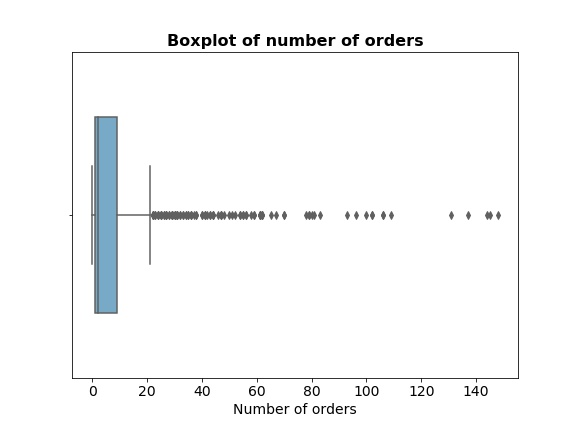
\includegraphics[width=\textwidth]{Images/boxplot_counts.jpg}
    \caption{Household Attributes}
    \label{fig:Household Attributes}
\end{figure}

The distribution plots for the exogenous variables can be found in the appendix. 

The scatter plot of the mean demand across all locations against the temperature visually display a slight positive relationship between temperature and demand. 

\section{Baseline Model}
In this section, we would build a simple baseline model. Following which, we would try other different spatial temporal time series models and compare the results to the baseline model. 

\subsection{Metric Used}
The main metric that would be used for comparison would be Mean Squared Forecast Error (MSFE), which is calculated by ....

\subsection{Train-Test Split}
Since there are many locations that have no demand or orders for the majority of the time period, the data is very sparse. Hence, to get a better idea of how our models would work, only locations with at least 50 non-zero counts across the time period would b used initially. The dataset was split into training and test set by considering the first 27 days as the training set and the next 7 days as the test set. Our training set would then have 162 demand data for each location and test set would have 42 demand data for each location. 

\subsection{ARIMA models}
Autoregressive Integrated Moving Average (ARIMA) models.....

\subsection{Baseline ARIMA Result}
As a baseline model, each of the locations was assessed individually and a suitable ARIMA model was built for each location. Auto-arima function from Python was used to implement this. The out-of-sample MSFE for this baseline model on the 42 locations is 58.80. 

\section{VAR Model}
Vector Autoregressive (VAR) models are....

VAR is commonly used in economics and financial time series. 

To validate if the multi-variate time series is stationary, the Johansen's test for cointegrating time series would be performed.
\begin{assumption}
The first assumption of a VAR model is....
\end{assumption}
\begin{assumption}
It is generally true...
\end{assumption}

\subsection{VARX Model}
VAR models can also be extended to include exogenous variables. 

\subsection{Model Checking}
To validate our model, the residuals....

\subsection{Results}
BigVAR library in R was used to implement the VAR models. The results from the VAR model without exogenous variables gives an out-of-sample MSFE of 46.641 on the 42 locations. 


\section{GLM Model}
\begin{assumption}
Generalised Linear Models (GLM) are.....
\end{assumption}
\begin{assumption}
An assumption is that the data follows a poisson process or a non-homogenous poisson process. 
\end{assumption}

\subsection{Model Checking}
To validate our model,

\subsection{Insights and Implementation}
Any findings from the results? If there are any benefits or issues in implementing the proposed model...
\section{Conclusion}
Conclude your efforts and main findings.

\section{Appendix}
Append extra plots, graphs, analysis, etc. \cite{Williamson2001}

%%%%%%%%%%%%%%%%%%%%%%%%%%%%%%%%%%%%%%%%%%%%%%%%%%%%%%%%%%%%
%%% Bibliography
%%%%%%%%%%%%%%%%%%%%%%%%%%%%%%%%%%%%%%%%%%%%%%%%%%%%%%%%%%%%
\bibliographystyle{apa} 
\bibliography{references}

\end{document}
